% -*- root: ../../main.tex -*
%!TEX root = ../../main.tex
% vim:textwidth=80 fo=cqt conceallevel=0


At the outset, it is worth mentioning that the focus of this chapter
is on the layer optimisation \emph{methodology} itself. The results
as such do not stand alone outside of the modelling universe with all
the inherent assumptions discussed thus far. Presently, the value added
by this work is its ready adaptability to industry through its modular
design. A numerical implementation in the form of a toolbox\footnote{The
\gls{bold} Toolbox is made available for download from GitHub. \\
\mbox{\href{https://github.com/ImperialCollegeESE/BOLD_Toolbox}{
\includegraphics
[width=0.025\textwidth]{github.pdf}}} \url{
https://github.com/ImperialCollegeESE/BOLD_Toolbox}} is also provided
which is immediately available for download and use by industry. This author
recommends that until the tool matures, cell manufacturers substitute their own
parameters and adjust other numerical coefficients suitably so that the toolbox
supplements, rather than supplants present empirical layer designs. Hence, the
results presented in this section must be interpreted in the backdrop of the
context within which the methodology was developed implying that the reader
must consciously strive to interpret all numerical values in \emph{relative} terms
of magnitude. To aid this thought process, this author chooses to deliberately
limit the discussion around the \emph{absolute} magnitude of numbers presented here.

\subsection{Modelling Platform and Preconditioning}

The thermally-coupled, \gls{p2d} electrochemical cell model used for
simulating each layer choice is implemented in MATLAB~\cite{matlab}, using
a heavily-modified version of the LIONSIMBA toolbox~\cite{Torchio2016}.
The work reported in this chapter helped to advance the toolbox from~v1.0x
to~v2.0. The updated computer codes to which this author heavily contributed,
is available from the project's official repository\footnote{LIONSIMBA~v2:
\mbox{\href{https://github.com/lionsimbatoolbox/LIONSIMBA}{
\includegraphics
[width=0.025\textwidth]{github.pdf}}} \url{
https://github.com/lionsimbatoolbox/LIONSIMBA}}.

The  rationale  behind  choosing  this  specific  software  to  implement  layer
optimisation  is  as  follows.  The LIONSIMBA~v1.0x  toolbox  has  already  been
validated against  the results of DUALFOIL~\cite{Dualfoil1998}  codes (which can
be considered as the present benchmark  standard). The toolbox is implemented in
the  MATLAB programming  language.  Since  this chapter  has  a strong  industry
focus,  the  omnipresence  of  MATLAB  in industry,  its  mature  code-base  and
familiarity  was  a strong  motivator  in  the  adoption  of this  toolbox.  The
simulation  speeds using  LIONSIMBA  have been  shown to  be  comparable to  the
FORTRAN  implementation  of  DUALFOIL,  primarily  owing  to  the  sophisticated
computation  of  the  analytical  Jacobian   of  the  system  through  automatic
differentiation~\cite{Torchio2016}.  In  addition  to  fundamental  enhancements
to   the  modelling   platform  presented   in~\cref{sec:numericalenhancements},
numerous  bug fixes  and  other  minor enhancements  to  the original  LIONSIMBA
code-base   have  been   provided  by   this  thesis   author.  The   interested
reader  may  peruse  these  from  the  \texttt{README.md}  file  hosted  on  the
\href{https://github.com/lionsimbatoolbox/LIONSIMBA}{project's  repository}. The
complete  parameter set  used  for  simulation of  this  model  is presented  in
table~\ref{tbl:lcoSimParamslayeropt}.  All  cells are  assumed  to  be in  their
equilibrium state prior to beginning of simulations.

% -*- root: ../../main.tex -*-
%!TEX root = ../../main.tex
% vim:nospell

\begin{table}[!htbp]
    \small
    \caption[%
    System-level simulation conditions \& thermal parameters of  an \glsfmtshort{lco} cell
    ]%
    {%
        Cell   parameters   and   system   conditions  for   a   simulating   an
        \glsfmtshort{lco} cell  with the  \gls{dfn} electrochemical model  and a
        lumped thermal model. The parameters  presented here when augmented with
        the  values  of  the  kinetic, geometric  and  transport  properties  of
        the  cell (from  \cref{tbl:lcoSimParamsSPMp2d}  represents the  complete
        information  required for  all  simulations in  this layer  optimisation
        framework.
    }%
    \label{tbl:lcoSimParamslayeropt}
    \vspace{-2.6229525pt}
    \begin{threeparttable}
        \centering
        \textbf{System Conditions} \\ \smallskip
        \begin{varwidth}[t]{0.48\linewidth}
            \begin{tabular*}{\textwidth}{@{} l @{\extracolsep{\fill}} S[table-format=1.2,table-space-text-pre=\Tnote{a} ,table-align-text-pre=false] @{}}
                \toprule
                \multicolumn{1}{@{}l}{Parameter} \\
                \midrule

                Lower cutoff cell voltage, $V_\text{min}$ (\si{\volt}) & \Tnote{a} 3.50   \\
                Upper cutoff cell voltage, $V_\text{max}$ (\si{\volt}) & \Tnote{b} 4.22   \\

                \bottomrule
            \end{tabular*}
        \end{varwidth}
        \hfill
        \begin{varwidth}[t]{0.48\linewidth}
            \begin{tabular*}{\textwidth}{@{} l @{\extracolsep{\fill}} S[table-format=2.2,table-space-text-pre=\Tnote{a} ,table-align-text-pre=false] @{}}
                \toprule
                \multicolumn{1}{@{}l}{Parameter} \\
                \midrule

                Target cell SOC for fast charge, $z^\ast$ \si{(\%)}                & \Tnote{c} 80.00 \\
                Cell upper temperature limit, $T_\text{max}$ \si{(\degreeCelsius)} & \Tnote{d} 55.00 \\

                \bottomrule
            \end{tabular*}
        \end{varwidth}

        \medskip
        \begin{tabular*}{\textwidth}{@{} l @{\extracolsep{\fill}} r @{}}
            \multicolumn{2}{c}{\textbf{Geometric Parameters}} \\
            \toprule
            \multicolumn{1}{@{}l}{Parameter} \\
            \midrule
            Surface area of pos.\ \& neg.\ electrode overlap within a layer, {$A_\text{elec}$} \si{(m^2)} & \textsuperscript{b}\num{4.19e-2}   \\
            Exterior pouch length, $L_\text{pouch}$ \si{(m)}                                              & \textsuperscript{e}\num{332.74e-3} \\
            Exterior pouch width, $W_\text{pouch}$ \si{(m)}                                               & \textsuperscript{e}\num{99.06e-3}  \\
            Exterior pouch height, $H_\text{pouch}$ \si{(m)}                                              & \textsuperscript{f}\num{10.00e-3}  \\
            Pouch material thickness, $T_\text{pouch}$ \si{(m)}                                           & \textsuperscript{g}\num{160.00e-6} \\
            \bottomrule
        \end{tabular*}
        \medskip
        \centering \textbf{Thermal Parameters} \\ \smallskip
        \resizebox{\textwidth}{!}{%
            \begin{tabular}{@{} l S[table-format=4.0,table-space-text-pre=\Tnote{m} ,table-align-text-pre=false] S[table-format=4.1,table-space-text-pre=\Tnote{m} ,table-align-text-pre=false] S[table-format=4.1,table-space-text-pre=\Tnote{m} ,table-align-text-pre=false] S[table-format=4.2,table-space-text-pre=\Tnote{m} ,table-align-text-pre=false] S[table-format=4.0,table-space-text-pre=\Tnote{m} ,table-align-text-pre=false] S[table-format=4.1,table-space-text-pre=\Tnote{m} ,table-align-text-pre=false] S[table-format=4.1,table-space-text-pre=\Tnote{m} ,table-align-text-pre=false] @{}}
                \toprule
                \multicolumn{1}{@{}l}{Parameter} & \multicolumn{1}{c}{Al.\ CC} & \multicolumn{1}{c}{Pos} & \multicolumn{1}{c}{Sep} & \multicolumn{1}{c}{Neg} & \multicolumn{1}{c}{Cu.\ CC} & \multicolumn{1}{c}{\ch{LiPF_6}} & \multicolumn{1}{r@{}}{Pouch}\\
                \midrule

                Sp.\ heat capacity, $c_j$ (\si{\joule\per\kilogram\per\kelvin})   & \Tnote{h} 903  & \Tnote{h} 1269.2 & \Tnote{h} 1978.2 & \Tnote{h} 1437.4 & \Tnote{h} 385  & \Tnote{h} 2055.1 & \Tnote{i} 1464.8 \\
                Density, $\rho_j$ (\si{\kilogram\per\meter\cubed})                & \Tnote{j} 2700 & \Tnote{k} 2291.6 & \Tnote{b} 1100.0 & \Tnote{j} 2660.0 & \Tnote{l} 8960 & \Tnote{j} 1290.0 & \Tnote{m} 1150.0 \\
                Activ.\ energy, diff. ${E_\text{act,s}}_j$ (\si{\joule\per\mole}) & {---}                   & \Tnote{p} 5000   & {---}                     & \Tnote{p} 5000   & {---}                   & {---}                     & \multicolumn{1}{c}{---}   \\
                Activ.\ energy, rxn. ${E_\text{act,k}}_j$ (\si{\joule\per\mole})  & {---}                   & \Tnote{p} 5000   & {---}                     & \Tnote{p} 5000   & {---}                   & {---}                     & \multicolumn{1}{c}{---}   \\

                \bottomrule
            \end{tabular}
        }
        \medskip
        \begin{tabular*}{\textwidth}{@{} l @{\extracolsep{\fill}} r @{}}
            \multicolumn{2}{c}{\textbf{Other Geometric/Cell-Level Parameters}} \\
            \toprule
            \multicolumn{1}{@{}l}{Parameter} \\
            \midrule

            Thickness of pos.\ current collector, $l_\text{Al}$ \si{(m)}                    & \textsuperscript{f}\num{15e-6}   \\
            Thickness of neg.\ current collector, $l_\text{Cu}$ \si{(m)}                    & \textsuperscript{p}\num{10e-6}   \\
            Total tab area, $A_\text{tabs}$ \si{(m^2)}                                      & \textsuperscript{b}\num{5.94e-3} \\
            Lumped heat transfer coefficient, $h$ (\si{\watt\per\meter\squared\per\kelvin}) & \textsuperscript{b}150           \\
            Initial electrolyte concentration, $c_\text{e,0}$ (\si{\mole\per\meter\cubed})  & \textsuperscript{q}1000          \\

            \bottomrule
        \end{tabular*}

        \medskip
        \begin{tabular*}{\textwidth}{@{} =P{7.5cm}  +l@{\extracolsep{\fill}}+c +r @{}}
            \multicolumn{4}{c}{\textbf{Spatial Discretisation}} \\
            \toprule
            \multicolumn{1}{@{}l}{Parameter} & \multicolumn{1}{l}{Pos} & \multicolumn{1}{c}{Sep} & \multicolumn{1}{r@{}}{Neg}\\
            \midrule

            Nodes, through-thickness (axial), $N_{\text{a}_j}$          & \num{40} & \num{40} & \num{40} \\
            Nodes, within spherical particle (radial), $N_{\text{r}_j}$ & \num{15} & ---      & \num{15} \\

            \bottomrule
        \end{tabular*}

        \medskip
        \vspace{-2.6229525pt}
        \begin{tablenotes}[para,flushleft]
            \begin{footnotesize}
            \item[a] Calculated as described in \cref{sec:cutoff}
            \item[b] Assumed
            \item[c] Ref.~\cite{Sae2010}
            \item[d] Ref.~\cite{Kizilel2009} \\
            \item[e] Converted from imperial units reported in~Ref.~\cite{GMBoltBatteryDims}
		    \item[f] Table~\romanletter{4} of~Ref.~\cite{Groger2015} \\
            \item[g] Sum of values in table~1 of~Ref.~\cite{Svens2013}
            \item[h] Ref.~\cite{Chen2005}
            \item[i] Computed from values of constituents (see~\cite{Svens2013}) using Ref.~\cite{martienssen2006springer} \\
            \item[j] Ref.~\cite{Guo2010}
            \item[k] Ref.~\cite{Jeon2011}
            \item[l] Ref.~\cite{Worwood2017,Song2000}
            \item[m] Ref.~\cite{Kim2009}
            \item[p] Ref.~\cite{Northrop2011}
            \item[q] Ref.~\cite{Subramanian2009}
            \end{footnotesize}
        \end{tablenotes}
    \end{threeparttable}
\end{table}



\subsection{\glsfmtshort{xeV} configurations}


% -*- root: ../../main.tex -*-
%!TEX root = ../../main.tex
% vim:nospell


\begin{table}[!htbp]
	\renewcommand{\thetable}{\arabic{table}a}
	\centering
	\caption{Acceleration test parameters (common across xEV platforms)}
	\label{tbl:CommonVehicleParams}
	\sisetup{table-format=3.2, table-number-alignment=center, table-space-text-pre=\textsuperscript{a}, table-space-text-post=\textsuperscript{a}, table-align-text-post=false}
	\begin{threeparttable}[t]
		\centering
		\begin{tabular}{@{} l  S @{}}
			\toprule
			Parameter \\
			\midrule

			% Coefficient of drag for xEV body, $C_\mathrm{d}$                           & {\makebox*{00}[r]{\tnote{a}}} 0.31                \\
			% Frontal area of xEV, $A_\mathrm{v}$ \si{(m^2)}                             & {\makebox*{00}[r]{\tnote{b}}} 2.40                \\
			% Acc.\ time specified by manufacturer, $t_\mathrm{f,man}$ \si{(s)}          & {\makebox*{00}[r]{\tnote{d}}} 6.50                \\
			% Acc.\ time dictated by standards, $t_\mathrm{f,std}$ \si{(s)}              & {\makebox*{00}[r]{\tnote{c}}} 6.00                \\
			% Speed, end of acc. (standards), $v_\mathrm{f,std}$ \si{(m.s^{-1})}         & {\makebox*{00}[r]{\tnote{e}}} 8.94                \\
			% Speed, end of acc. (manufacturer), $v_\mathrm{f,man}$ \si{(m.s^{-1})}      & {\makebox*{0}[r]{\tnote{f}}} 26.82                \\
			% Base speed of  xEV, $v_\mathrm{b}$ \si{(m.s^{-1})}                         & {\makebox*{\hspace*{0.5mm}0}[r]{\tnote{e}}} 13.41 \\
			% Air density at acc.\ test conditions, $\rho_\mathrm{air}$ \si{(kg.m^{-3})} & {\makebox*{\hspace*{0.5mm}00}[r]{\tnote{f}}} 1.20 \\
			% Drivetrain efficiency, $\eta_\mathrm{dt}$                                  & {\makebox*{00}[r]{\tnote{g}}} 0.75                \\
			% Payload, $M_\mathrm{p}$ \si{(kg)}                                          & {\hspace*{0.00005mm}{\tnote{c}}} 150.60 \\
			% Rolling resistance coefficient of road surface, $C_\mathrm{r}$             & {\makebox*{00}[r]{\tnote{f}}} 0.01                \\
			% Road gradient, $Z$                                                         & {\makebox*{00}[r]{\tnote{g}}} 0.00                \\

			Coefficient of drag for xEV body, $C_\mathrm{d}$                           & 0.31   {\tnote{a}} \\
			Frontal area of xEV, $A_\mathrm{v}$ \si{(m^2)}                             & 2.40   {\tnote{b}} \\
			Acc.\ time specified by manufacturer, $t_\mathrm{f,man}$ \si{(s)}          & 6.50   {\tnote{d}} \\
			Acc.\ time dictated by standards, $t_\mathrm{f,std}$ \si{(s)}              & 6.00   {\tnote{c}} \\
			Speed, end of acc. (standards), $v_\mathrm{f,std}$ \si{(m.s^{-1})}         & 8.94   {\tnote{e}} \\
			Speed, end of acc. (manufacturer), $v_\mathrm{f,man}$ \si{(m.s^{-1})}      & 26.82  {\tnote{f}} \\
			Base speed of  xEV, $v_\mathrm{b}$ \si{(m.s^{-1})}                         & 13.41  {\tnote{e}} \\
			Air density at acc.\ test conditions, $\rho_\mathrm{air}$ \si{(kg.m^{-3})} & 1.20   {\tnote{f}} \\
			Drivetrain efficiency, $\eta_\mathrm{dt}$                                  & 0.75   {\tnote{g}} \\
			Payload, $M_\mathrm{p}$ \si{(kg)}                                          & 150.60 {\tnote{c}} \\
			Rolling resistance coefficient of road surface, $C_\mathrm{r}$             & 0.01   {\tnote{f}} \\
			Road gradient, $Z$                                                         & 0.00   {\tnote{g}} \\

			\bottomrule
		\end{tabular}
        \begin{tablenotes}[para,flushleft]
        \item[a]Ref.~\cite{HybridCars2017Drag}
        \item[b]Calculated from typical \gls{bev} dimensions in~\cite{BoltDimensions}
        \item[c]Ref.~\cite{ETANTP002-2004}
        \item[d]Ref.~\cite{BoltOverview}
        \item[e]Ref.~\cite{Liu2016a}
        \item[f]Ref.~\cite{EmadiElectric}
        \item[g]Assumed
        \end{tablenotes}
	\end{threeparttable}
\end{table}


Tables~\ref{tbl:CommonVehicleParams} and~\ref{tbl:UniqueVehicleParams}  show the
\gls{xeV}  parameters  used  in  simulations. In  this  author's  analysis,  the
power  demands on  the battery  pack  during normal  operation are  found to  be
significantly  lower than  that  experienced  during the  two  extreme cases  of
discharging  and charging  \viz{} \emph{acceleration}  and \emph{fast  charging}
respectively. For  instance, \SI{50.83}{\kilo\watt} is the  peak discharge power
while \SI{14.20}{\kilo\watt} is the median  discharge power for various standard
drive  cycles.  Even with  the  assumption  that \SI{100}{\percent}  of  braking
energy  can  be  recovered,  the  peak  and  median  charging  powers  are  only
\SI{43.13}{\kilo\watt} and \SI{26.03}{\kilo\watt}  respectively. Considering the
acceleration  parameters  in~\cref{tbl:CommonVehicleParams}  for  the  \gls{bev}
pack, \SI{181.45}{\kilo\watt}  is the  power requirement  for acceleration  of a
fixed vehicle  mass on a  flat road  surface. Four distinct  fast-charging power
levels \viz{} \SI{50}{\kilo\watt}, \SI{80}{\kilo\watt}, \SI{110}{\kilo\watt} and
\SI{130}{\kilo\watt}  are considered  in this  study.  This is  in adherence  to
the  minimum  and maximum  values  of  level~3  rating  as suggested  by  Yilmaz
and~Krein~\cite{Yilmaz2012}. Furthermore, near-term fast charging goals laid out
in  literature~\cite{Ashique2017,Srdic2016} and  the  peak  power capability  of
charging infrastructure further justify these choices.

% -*- root: ../../main.tex -*-
%!TEX root = ../../main.tex
% vim:nospell


\begin{table}[!htbp] % Parameters unique to each of the BEV & PHEV
	% \addtocounter{table}{-1}
	% \renewcommand{\thetable}{\arabic{table}b}
	\caption{Acceleration test parameters (specific to each \glsfmtshort{xeV})}
	\label{tbl:UniqueVehicleParams}
	\centering
    \sisetup{table-format=4.1, table-number-alignment=center, table-space-text-pre=\textsuperscript{a}, table-align-text-pre=false}
	\begin{threeparttable}[t]
		\begin{tabular*}{0.72\textwidth}{@{} l @{\extracolsep{\fill}}  S S @{}}	% Works with Tnote
			\toprule
			\multicolumn{1}{@{} l}{Parameter} & \multicolumn{1}{c}{BEV} & \multicolumn{1}{c@{}}{PHEV} \\
			\midrule

			Mass of xEV chassis, $M_\mathrm{c}$ \si{(kg)}               & \Tnote{a} 1340.0 & \Tnote{b} 1438.0 \\
			Mass of pack overhead (w/o cells), $M_\mathrm{o}$ \si{(kg)} & \Tnote{a} 196.4  & \Tnote{c} 65.5   \\
			Upper cutoff SOC of cell, $z_\mathrm{max}$ \si{(\%)}        & \Tnote{d} 95.0   & \Tnote{d} 90.0   \\
			Lower cutoff SOC of cell, $z_\mathrm{min}$ \si{(\%)}        & \Tnote{d} 5.0    & \Tnote{e} 30.0   \\

			\bottomrule
		\end{tabular*}
		\begin{tablenotes}[para,flushleft]
		\item[a]Calculated based on~\cite{ChevyBoltSpecs}
		\item[b]Calculated based on~\cite{motortrendEcotec,ChevyBoltSpecs}
		\item[c]Calculated (see sections~\ref{sec:layerdependentvehiclemass} \& \ref{sec:massofonecell})
		\item[d]Assumed
		\item[e]Ref.~\cite{EmadiElectric}
		\end{tablenotes}

	\end{threeparttable}
\end{table}


For  the  acceleration  tests,  the  initial cell  \gls{soc}  has  been  set  to
\SI{40}{\percent}.  This  is  in  conformity with  the  test  criterion  $(50\pm
10)$~\%  of  the  SAE~J1666   standard~\cite{Sae2010}.  By  choosing  the  worst
case  starting  \gls{soc} \ie{}  \SI{40}{\percent},  a  conservative design  can
be  achieved.  The  chassis  mass  of  the  vehicle  as  well  as  the  mass  of
two  passengers   at  75.3  kg   each~\cite{Sae2010}  is  considered   for  both
\gls{xeV}  platforms. The  pack mass  is  computed as  a function  of number  of
layers  as described  in~\cref{sec:layeroptframework}. The  vehicle manufacturer
General  Motors  Inc.\ suggests  the  mass  value of  the  GM  Ecotec series  of
engines~\cite{motortrendEcotec} to  use for the  \gls{phev} which consists  of a
range-extending  \gls{ice}.  The  mass  of  the  Bolt  \gls{bev}  pack  reported
in~\cite{ChevyBoltSpecs} minus  the computed mass  of the overall cells  used in
the pack  gives the overhead mass  of the \gls{bev} pack.  The \gls{phev} pack's
overhead mass  is determined by suitably  scaling the mass by  the proportion of
reduction in the number of cells used.

For the \gls{bev}  platform, a fast-charging scheme operated on  a \gls{cp} mode
with an initial  \gls{soc} of \SI{20}{\percent} is employed. In  the case of the
\gls{phev}, an initial \gls{soc}  of \SI{30}{\percent} (\SI{10}{\percent} higher
than that for \gls{bev}) is used. This facilitates a smaller \gls{soc} window by
taking  into account  the higher  number  of charge-discharge  cycles which  are
typical with \gls{phev}  designs~\cite{Maksimovic2012}. Both \gls{xeV} platforms
are fast  charged to a target  \gls{soc} of \SI{80}{\percent} in  \gls{cp} mode.
This \gls{soc} value corresponds to the end-of-charge target in level~3 charging
standards~\cite{SAECharging2011}.

\subsection{Acceleration studies}

For both vehicle platforms under study, the acceleration at a worst-case rate of
\SI{4.13}{\meter\per\second\squared} is assumed for simulation. This corresponds
to the  manufacturer's acceleration specifications  for the \gls{bev}  listed in
\cref{tbl:CommonVehicleParams}.  The  acceleration  rate  corresponding  to  the
SAE~J1772 standards is lower than this  rate. Therefore, to obtain a robust cell
design, the higher of the two acceleration rates needs to be considered.

\Cref{tbl:accResults}  gives the  simulation  results  for various  combinations
of  $(T_\text{init},  T_\text{sink})$  for  both the  \gls{bev}  and  \gls{phev}
platforms. The following discussion is applicable for both vehicular platforms.

% -*- root: ../../main.tex -*-
%!TEX root = ../../main.tex
% vim:nospell

\begin{table}[htb!]
    \caption{\glsfmtshort{xeV} acceleration test results}
    \label{tbl:accResults}
    \centering
	\begin{tabular}{c c c}
        \toprule
        \multicolumn{1}{@{} l}{\makecell{($T_\text{init},T_\text{sink}$) \\ \footnotesize (degC)}} & \makecell{$n^\text{acc}_\text{opt}$ \\ \footnotesize \glsfmtshort{bev}}&  \multicolumn{1}{c @{}}{\makecell{$n^\text{acc}_\text{opt}$ \\ \footnotesize \gls{phev}}}  \\
        \midrule

        (38,5)  & \num{21} & \num{55} \\
        (38,49) & \num{21} & \num{57} \\
        (25,25) & \num{23} & \num{63} \\
        (15,5)  & \num{27} & \num{69} \\

        \bottomrule
    \end{tabular}
\end{table}


The  specific combinations  of temperatures  for traversing  the thermal  design
space are  chosen following the  SAE~J1772 guidelines. The high  power densities
resulting from  low numbers of layers  lead to large overpotentials  causing the
cell's terminal voltage  to drop lower down than  $V_\text{min}$, thereby unable
to satisfy acceleration requirements.  However, at higher $T_\text{init}$, owing
to the  reduction in overpotentials, a  larger voltage overhead is  available to
accommodate the  internal polarisation  drop. For all  temperature combinations,
the largest deviation from $T_\text{init}$ experienced  by a \gls{bev} cell is a
\SI{0.48}{\degreeCelsius}  increase. Consequently,  it can  be concluded  that a
single isolated acceleration event does not heat the \gls{bev} battery pack, and
therefore the cell  temperature remains close to that of  the initial value. The
\gls{phev} cell  experiences higher  power levels  and although  its temperature
increases  much  higher  than  the corresponding  \gls{bev}  cell,  the  maximum
temperature during acceleration  run remains well below the  upper cutoff limit.
Furthermore, even  for the worst  case simulation  run, the cell's  \gls{soc} is
depleted only by  a maximum value of \SI{0.32}{\percent} for  the \gls{bev} cell
and by a slightly higher value for the \gls{phev} cell.

The foregoing  discussion has revealed  that the lower cut-off  voltage strongly
influences  layer   configuration  for   acceleration  tests.   Therefore,  when
considering acceleration requirements, $n = 27$ and $n=69$ represent the optimal
layer choices for the \gls{bev} and \gls{phev} platforms respectively .

\subsection{Fast charging studies}

\begin{figure}[p]
    \begin{minipage}[t]{\textwidth}
        \centering
        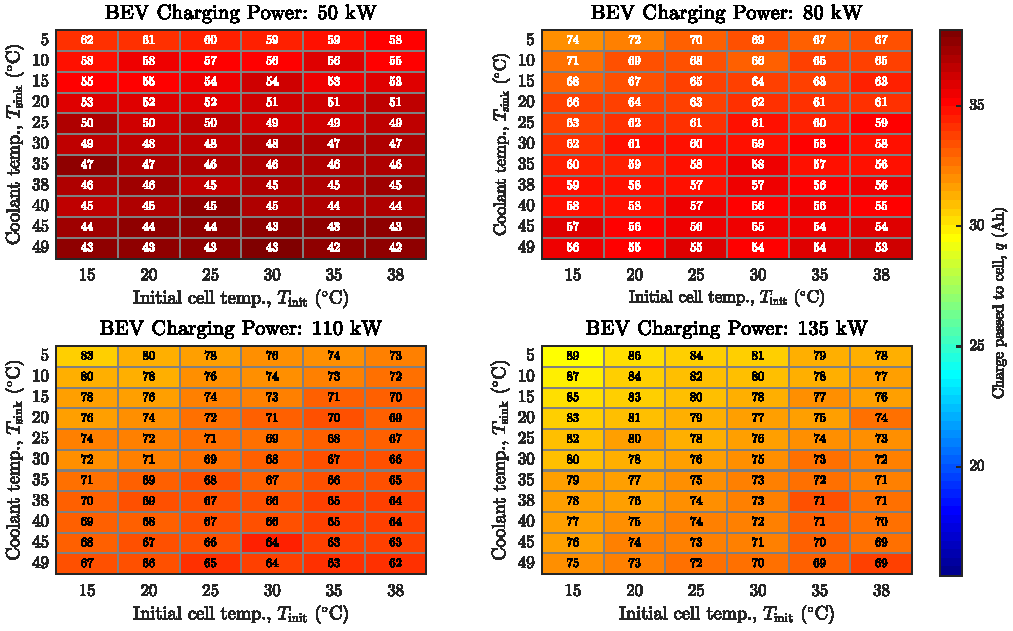
\includegraphics[width=\textwidth]{fig_generate_heatmap_BEV}
        \captionsetup{labelsep=note}
        \caption[Optimal cell layer configurations for the \gls{bev}, presented for a range of fast charging powers and thermal conditions]{Optimal cell layer configurations for the \gls{bev}}
        \label{fig:fig_generate_heatmap_BEV}
        \setcounter{footnote}{9}
        \vspace*{\floatsep}
        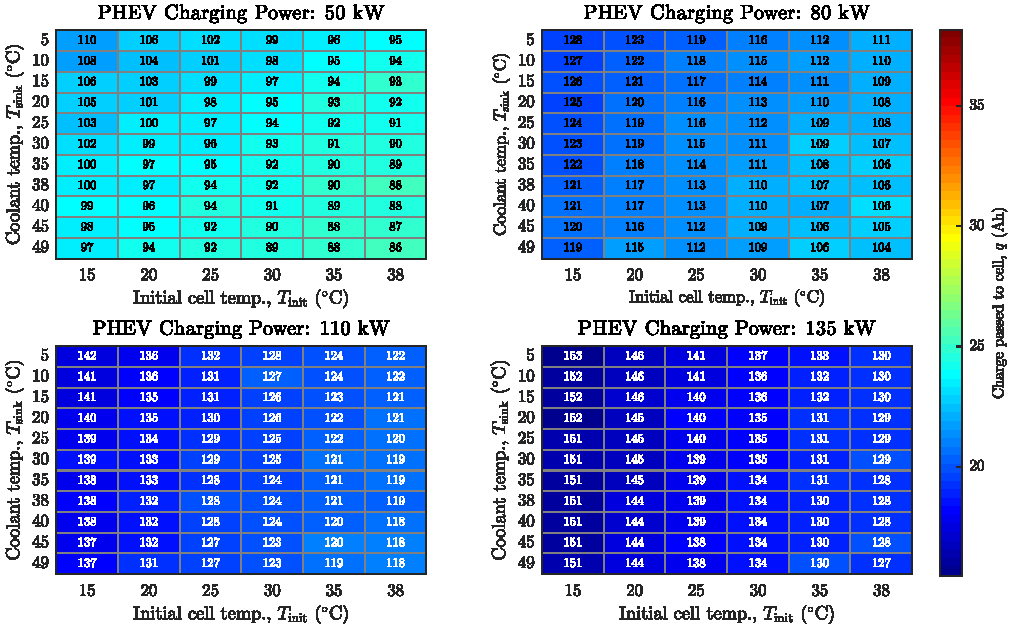
\includegraphics[width=\textwidth]{fig_generate_heatmap_PHEV}
        \caption[Optimal cell layer configurations for the \gls{phev}, presented for a range of
        fast charging powers and thermal conditions]{Optimal cell layer configurations for the \gls{phev}}
        \label{fig:fig_generate_heatmap_PHEV}
        \mpfootnotes[1]
        \footnote{These figures was created by \mbox{Ian Campbell} who asserts copyright,
            with intellectual contributions from and the right to use asserted by
        \mbox{Krishnakumar Gopalakrishnan}.}
    \end{minipage}
\end{figure}

Figures~\ref{fig:fig_generate_heatmap_BEV}
and~\ref{fig:fig_generate_heatmap_PHEV} show  the results produced by  the layer
optimisation framework  for the \gls{bev} and  \gls{phev} platforms respectively
when considering fast charging requirements. Each heat~map in these figures show
the optimal  number of  layers~$n^\text{fastchg}_\text{opt}$ for  every possible
combination  of initial  and ambient  temperatures for  four different  charging
powers. In each case, the  values of $n^\text{fastchg}_\text{opt}$ correspond to
the  temperature  combination  \mbox{$(T_\text{init},T_\text{sink})  =  (15,  5)
\si{\degreeCelsius}$}  as  shown  in  \cref{fig:fig_generate_heatmap_BEV}.  This
represents the  least number of  layers required to  fast charge the  pack under
\gls{cp} conditions until  the target \gls{soc} is reached.  The charging scheme
additionally considers the constraint that the cell temperature must stay within
\mbox{$T_\text{max}=  \SI{55}{\degreeCelsius}$}. Furthermore,  its voltage  must
remain less than or equal  to \mbox{$V_\text{max} = \SI{4.22}{\volt}$}. Finally,
the charging algorithm is plating-aware \ie{}  the charging stops as soon as the
concentration at the particle surface reaches the maximum possible concentration
limit, thereby preventing  lithium plating at the surface  of negative electrode
particles.


Thus,   using    the   model-based    design   strategy   presented    in   this
chapter,   an   effective    cell   design   is   achieved    which   helps   to
maximise   energy   density  and   \gls{bev}   range,   without  forgoing   fast
charging   power    targets.   From   figures~\ref{fig:fig_generate_heatmap_BEV}
and~\ref{fig:fig_generate_heatmap_PHEV},       it       is       seen       that
$n^\text{fastchg}_\text{opt}$  increases with  increase in  the charging  power.
This is because,  as the charging power increases, the  minimum number of layers
required to maintain  the cell voltage below the maximum  permissible value also
increases.  This requires  higher interfacial  surface area  to accommodate  the
increased  power demand.  Furthermore, rapid  surface saturation  occurs due  to
steep  concentration  profiles in  the  negative  electrode particles  when  the
charging power is  high which causes plating. With higher  layers, the resulting
electrodes  are thinner,  thereby allowing  faster diffusion  of lithium  in the
solid  particles  and  avoiding  steep concentration  gradients  in  them.  This
suggests that the number of layers must be large enough to prevent plating.

\Cref{fig:fig_CapacityQuadrants} shows the nominal  capacity of cells and charge
passed versus  the number of  layers during fast  charging. In these  plots, the
theoretical  capacity~$Q_\text{n}$ of  the cell  versus the  layer count~$n$  is
represented by the linear downward-sloping line.

\begin{figure}[!bp]
    \begin{minipage}[t]{\textwidth}
        \centering 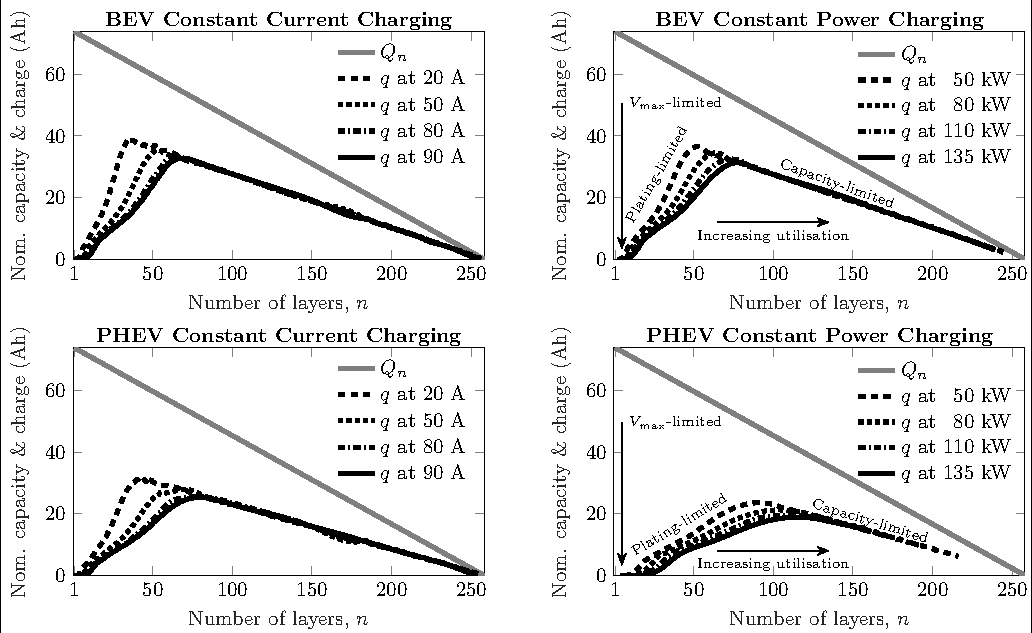
\includegraphics[width=\textwidth,trim=4 2 3 4,clip]{fig_capacity_quadrants.pdf}
        \captionsetup{labelsep=note}
        \caption[
        Nominal capacity and charge passed versus layer count for ---
        \emph{a}) constant current  charging and \emph{b}) constant power  charging
        ]
        {
            The plots in the right column show the nominal cell capacity and charge passed
            during \gls{xeV} \gls{cp} charging. Increased rate capability and cell utilisation are positively
            correlated with $n$, while the maximum-$q$ layer configuration clearly shifts to higher
            values of $n$ with increasing charging powers. The plots in the left column depict
            galvanostatic charging scenarios at various currents to highlight the similarity with the
            \gls{cp} process. All data obtained at $T_\text{init} =$ \SI{25}{\degreeCelsius},
            $T_\text{sink} =$ \SI{25}{\degreeCelsius}.
        }
        \label{fig:fig_CapacityQuadrants}
        \mpfootnotes[1]
        \footnote{This figure was created by \mbox{Ian Campbell} who asserts copyright,
            with intellectual contributions from and the right to use asserted by
        \mbox{Krishnakumar Gopalakrishnan}.}
    \end{minipage}
\end{figure}

For any layer  choice, $Q_\text{n}$ therefore represents the upper  bound on the
charge  that can  be  passed  during charging.  For  both  constant current  and
constant power  charging, the locus  of the  actual charge passed~$q$  lies much
below  this theoretical  nominal capacity.  For very  low layer  counts, as  the
number of layers  decreases, the power density drops rapidly  which implies that
the rate of heating  is low. This allows for more charge  to be passed. However,
at  ultra-low  layer  counts,  the  overpotential due  to  the  cell's  internal
resistance is  quite high. Therefore,  hitting the  upper bound on  the terminal
voltage is the reason for the failure  of these layer choices. This is indicated
by the narrow $V_\text{max}$-limited region in \cref{fig:fig_CapacityQuadrants}.
For an intermediate range of layer  choices, the rate of power-density drop with
layer count begins to flatten, thereby  leading to a plating-limited region. For
these layer choices,  the surface concentration starts to  exceed the saturation
value  before  any thermal  or  voltage  limits  are reached.  Finally,  further
increasing  the layer  count beyond  an intermediate  optimal value  leads to  a
linear drop in the cell's charge accepting capability. During fast charging with
the chosen power levels, although these  layer choices do not reach the thermal,
voltage or concentration limits, they are  unable to attain the target \gls{soc}
of \SI{80}{\percent}.  This is simply due  to the lower nominal  capacity of the
these cells. There  is no benefit whatsoever in designing  cells in this region.
\Cref{fig:fig_CapacityQuadrants} provides  clues to  the design engineer  on the
degree  of optimisation  that can  be achieved  by careful  design choices.  For
instance, by tuning certain design parameters, such as using electrode materials
capable  of  operating at  higher  plating  voltage  or with  higher  saturation
concentration, the optimisation  point can be appropriately adjusted  as per the
application's demands.


From  the results  discussed thus  far, it  is evident  that it  is the  thermal
environment  that  governs   the  optimal  cell  layer   configuration  in  both
acceleration and fast charging studies and for both vehicular platforms. For all
charging powers simulated, $n^\text{fastchg}_\text{opt}$  is the highest for the
coldest temperature  combination \mbox{$(T_\text{init},T_\text{sink}) =  (15, 5)
\si{\degreeCelsius}$}. This is due to  the slow rate of electrochemical reaction
and diffusion  at cold  temperatures. The thinner  electrodes from  using higher
layer count enable fast charging without saturating the surface of the electrode
particles. For the  fast charging scenarios considered here,  the optimal number
of layers to use  is 89~for the \gls{bev} cell and  153~for the \gls{phev} cell.
The globally optimal  layer choice to be  used for cell design  is therefore the
higher of the two values corresponding  to acceleration and fast charging cases.

Therefore, this model-based design framework recommends the use of 89~layers for
the cells to be  used in the \gls{bev} platform and 153~layers  for the cells to
be used in the \gls{phev} platform.  This concludes the discussion of results of
this chapter as well as all design-related aspects of this thesis.

